\section{Concurrency}

\subsection{Motivation}
\begin{itemize}
  \item Praktische Programme führen meist mehrere Arbeiten "`gleichzeitig"' aus. 
  \item Diese Nebenläufigkeit kann implementiert werden durch\ldots
  \begin{itemize}
    \item Quasi-Parallelität durch Betriebssystem $\rightarrow$ Synchronisation
    nötig, da auf gemeinsame Ressourcen zugegriffen wird
    \item Echte Parallelität durch Mehrprozessorsystem
  \end{itemize}
\end{itemize}
Richtwert: Aufgaben welche \textbf{länger als 100ms} dauern, sollten in den Worker-Thread ausgelagert werden.\\
Beispiele:
\begin{itemize}
  \item Webserver soll mehrere Requests gleichzeitig bearbeiten können.
  \item Embedded Systeme bearbeitet mehrere Aufgaben gleichzeitig.
\end{itemize}

\subsection{Parallel VS Concurrent computing}
\begin{multicols}{2}
  Parallel Computing (Multicore)
  \begin{itemize}
    \item Ausf\"uhrung von verschiedenen Aufgaben werden zur selben Zeit erledigt.
    \item Nur bei Multiprozessor-Controller m\"oglich
  \end{itemize}
\vfill\null
\columnbreak
  Concurrent Computing (Singlecore)
  \begin{itemize}
    \item Ausf\"uhrung scheint nur parallel abzulaufen
    \item Verschiedene Aufgaben werden bestimmte Zeitpunkte durch Scheduler zugeteilt
    \item Nur eine Aufgabe wird im Moment bearbeitet
    \item Realisierbar mit single- und multicore- Prozessoren
  \end{itemize}
  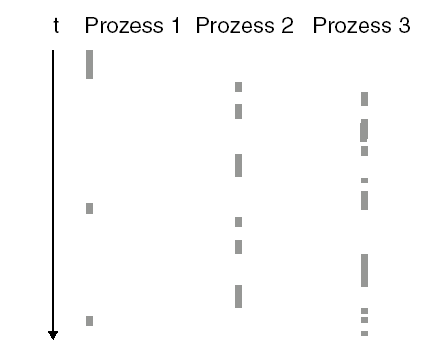
\includegraphics[width=5cm]{images/Concurrency/Quasiparallelitaet.png}
\end{multicols}

\textbf{Nachteile von Nebenläufigkeit}
\begin{itemize}
  \item  Concurrency (mit Prozessen, Tasks, Threads) kostet immer \ldots
  \begin{itemize}
    \item \ldots Stack
    \item \ldots Kontext switch
    \item \ldots Zugriffe auf gemeinsame Ressourcen muss synchronisiert werden.
  \end{itemize}
  \item  Komplexität steigt. Sequentielle Programme sind einfacher zu verstehen als parallele.
\end{itemize}
Concurrency nur dann einsetzen, wenn wirklich ein nutzen vorhanden ist.

\newpage

\subsection{POSIX Thread programming}
\begin{multicols}{2}
\subsubsection{UNIX Process}
\begin{itemize}
  \item heavyweight process (Erstellt vom Betriebssystem)
  \item Prozesse brauchen einen grossen Overhead und enthlaten Informationen über die Programmressourcen und Programmausführungszustände, miteinbezogen:
  Process ID, process group ID, user ID, group ID, Environment, Program instrcutions, registers, stack, heap, file descriptor, signal actions, shared libraries, interr-process communication tools
\end{itemize}
\vfill\null
\columnbreak
\subsubsection{UNIX Thread}
\begin{itemize}
  \item Lightweight "process"
  \item Threads benutzen und existieren mit den Prozessen
  \item Ein Thread hat denselben Adressraum wie die anderen Threads im selben Prozess
  \item Threads sind \textit{sceduable} vom Betriebssystem
  \item Unabhängige Instruktionen können simultan verlaufen
  \item Ein Thread beinhaltet: stack pointer, schudeling properties, set of pending and blocked signals, thread specific data
  \item Concurrent Computing werden mit Threads realisiert
\end{itemize}
\end{multicols}

\subsubsection{Process vs Thread UNIX}
\begin{center}
  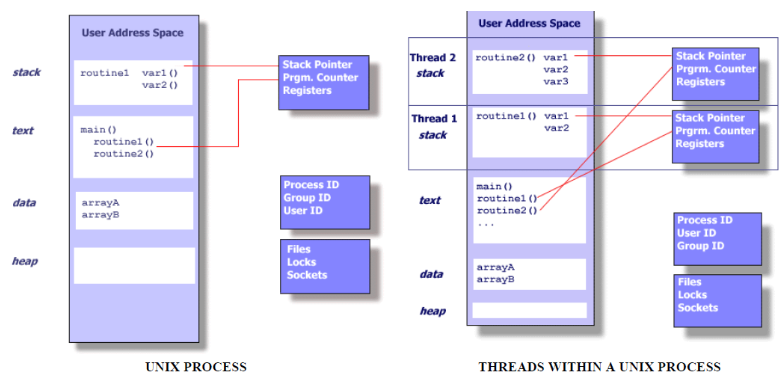
\includegraphics[width=0.8\textwidth]{images/Concurrency/ProcessVsThread.png}
\end{center}

\subsubsection{Thread Summary}
Ein Thread \ldots
\begin{itemize}
  \item \ldots exisitert während einem Prozess und benutzt die Prozessressourcen
  \item \ldots bleibt in seinen unabhängigen flow control solange der Prozess exisitert
  \item \ldots dupliziert nur die notwendigen Ressourcen
  \item \ldots teilt gegebenfalls Prozessressourcen mit anderen Threads
  \item \ldots stirbt wenn der Prozess stirbt
\end{itemize}

\newpage

\subsubsection{pthread API}
\begin{itemize}
  \item Routinen mit der pthread-API beginnen mit \textbf{pthread\_}
  \item Der Header lautet \textbf{pthread.h}
  \item Kompilieren und Linken \textbf{-pthread}
  \item link command für IDE \textbf{-lpthread}
\end{itemize}

\subsubsection{Starten und Terminieren}
\begin{lstlisting}
  #include <pthread.h>
  void* threadFunction(void* arg);
  int main(void)
  {
    pthread_t myT;
    int ret = pthread_create(&myT, 0, threadFunction, 0);
    if (ret)
    { // handle error
      return -1;
    }
    while (1) // endless loop
    {}
    return 0;
  }
  void* threadFunction(void* arg)
  { // implement this
    return 0;
  }
\end{lstlisting}

\subsubsection{Warten}
\begin{lstlisting}
#include <pthread.h>
void* threadFunction(void* arg);
int main(void)
{
  pthread_t myT;
  int ret = pthread_create(&myT, 0, threadFunction, 0); // only starts and returns
  if (ret)
  { // handle error
    return -1;
  }
  ret = pthread_join(myT, 0);
  if (ret)
  { // handle error
    return -1;
  }
    return 0;
}
void* threadFunction(void* arg)
{ // implement this
  return 0;
}
\end{lstlisting}

\newpage

\subsubsection{Join}
\begin{multicols}{2}
  \begin{lstlisting}
    #include <pthread.h>
    #include <stdio.h>
    #include <unistd.h>
    void* printDashes(void* arg);
    int main(void)
    {
      pthread_t dasher;
      printf("start");
      pthread_create(&dasher, 0, printDashes, 0); // fork
      pthread_join(dasher, 0); // join
      printf("end\n");
      return 0;
    }
    void* printDashes(void* arg)
    {
      for (int i=0; i<20; ++i)
      {
        usleep(40000);
        putchar('-');
        fflush(stdout); // write character-wise, don't buffer
      }
      return 0;
    }
    \end{lstlisting}
\vfill\null
\columnbreak
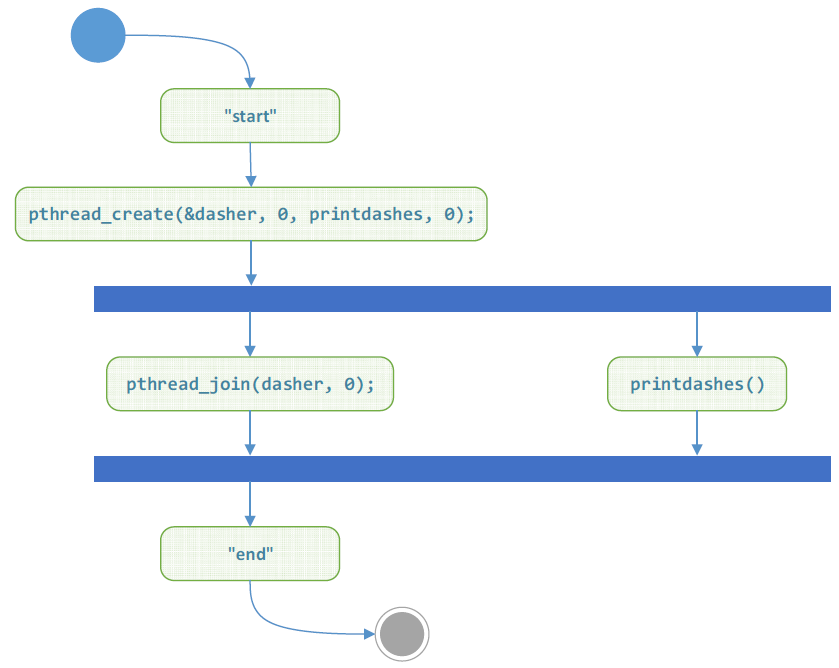
\includegraphics[width=0.5\textwidth]{images/Concurrency/pthreadJoin.png}
\end{multicols}

\subsubsection{Thread-safeness}
\textit{Thread-safeness} beschreibt die Eigenschaft einer Applikation, welche mehrere Threads 
simultan ausführen kann, ohne Fehlzugriffe auf \textit{shared data} oder eine \textit{race-condition} zu erzeugen.\\
Beispielverhalten einer Applikation mit mehreren erzeugten Threads, welche auf dieselben Bibliotheken zurückgreifen:
\begin{itemize}
  \item Bibliothek-Routine modifiziert eine globale Struktur oder lokaler Speicher
  \item Threads können gleichzeitig die Globalen Strukturen oder Daten bearbeiten
  \item Thread-safe ist nur vorhanden, wenn die Threads synchronisiert werden und somit kein \textit{data corruption} entsteht
\end{itemize}

\newpage

\subsection{Synchronisation}
\textbf{Kritischer Abschnitt}\\
Codebereich, in dem nebenläufige oder parallele Prozesse auf gemeinsame Ressourcen zugreifen. Zu jeder 
Zeit darf sich höchstens ein Prozess im kritischen Abschnitt befinden.
\\
Der exklusive Zugriff durch höchstens einen Prozess wird mittels gegenseitigem Ausschluss (mutual 
exclusion, Mutex) sichergestellt.

\subsubsection{mutual exclusion}
\begin{multicols}{2}
  \begin{itemize}
    \item Bei der Zugriffüberprüfung wird gewartet, bis der Zugang frei wird
    \item Beim Sperren wird das Signal auf Rot gesetzt, damit nur ein Prozess im kritischen Abschnitt sein kann \textbf{(Ist kein busy-waiting!)}
    \item Beim Freigeben wird das rote Signal wieder gelöscht
  \end{itemize}
  \vfill\null
  \columnbreak
  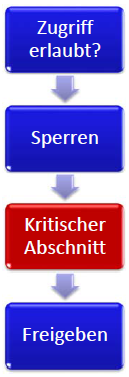
\includegraphics[width=0.1\textwidth]{images/Concurrency/Loesungsstruktur.png}
\end{multicols}
Forderungen an die Synchronisation:
\begin{enumerate}
  \item Keine zwei Prozesse gleichzeitig im kritischen Abschnitt
  \item Keine Annahmen über die Anzahl Prozesse bzw. die Abarbeitungsgeschwindigkeit
  \item Ein Prozess darf ausserhalb des kritischMit Deadlock wird die Situation bezeichnet, bei der sich zwei Prozesse gegenseitig blockierenen Abschnitts keine anderen Prozesse blockieren
  \item Prozesse am Eingang des kritischen Abschnitts müssen diese betreten dürfen (fairness condition)
\end{enumerate}

\subsubsection{Semaphoren}
Der Zutritt in einen kritischen Abschnitt wird als \textbf{Semaphor} bezeichnet. \textit{Semaphore} ist ein spezieller Name für ein Signal.
Programmiertechnische Lösung ist das \textit{RAII}\\
\begin{multicols}{2}
  \textbf{Atomare Operationen (nicht unterbrechbar)}
  \begin{itemize}
    \item P(s) Passieren: Beim Eintritt in CS(waitFor)
    \item V(s) Verlassen: Beim Austritt aus CS (send)
  \end{itemize}
  \vfill\null
  \columnbreak
  \textbf{Probleme von Semaphoren}
  \begin{itemize}
    \item Für jedes P(s) braucht es ein V(s)
    \item Probleme wenn V(s) mit if-Bedingung realisiert
    \item Komplikationen mit Exception-Handling können auftreten
  \end{itemize}
\end{multicols}

\subsubsection{Wichtige Begriffe}
  \begin{centering}
  \begin{tabular}{| p{6cm} | p{6cm} | p{6cm} |}
    \hline\textbf{Busy Waiting} & \textbf{Starvation} & \textbf{Deadlock}\\
    Beim Busy Waiting wartet mann aktiv in einer Schleife und brauchen unnötigerweise Prozessorleistung. Lösung: sleep und wake-up.&
    Mit Starvation wird der Zustand bezeichnet, bei dem ein Prozess nie dran kommt (er verhungert). Fairness-Condition verhindert dies.&
    Mit Deadlock wird die Situation bezeichnet, bei der sich zwei Prozesse gegenseitig blockieren. Lösung: Reihenfolge festlegen.\\\hline
  \end{tabular}
  \end{centering}

\subsubsection{Mutex}
\begin{lstlisting}
  static volatile int val = 0; // shared resource
  static pthread_mutex_t valMtx;
  int main(void)
  {
    pthread_t t;
    pthread_mutex_init(&valMtx, 0); // init mutex
    pthread_create(&t, 0, threadRoutine, 0);
    pthread_join(t, 0);
    pthread_mutex_destroy(&valMtx); // destroy mutex
    return 0;
  }
  void* threadRoutine(void* arg)
  {
    while (1)
    {
      // non critical section
      pthread_mutex_lock(&valMtx); // start of critical section
      // critical section; access shared resource
      pthread_mutex_unlock(&valMtx); // end of critical section
      // non critical section
    }
  }
\end{lstlisting}

\subsection{POSIX Threads programming}
Für UNIX Systeme wurde eine standardisierte C-Bibliothek von IEEE spezifiziert oder in kurz \textit{pthread}. 

\subsubsection{condition variable}
Duch eine \textit{condition variable} können Informationen zwischen Threads kommuniziert werden.
\begin{itemize}
  \item Mutexes implementiert die Synchronisierung
  \item Condition variables erlauben Threads zu synchronisieren
  \item Ohne condition variable muss gepollt werden
  \item condition variable wird immer im zusammenhang mit mutex lock verwendet.
\end{itemize}
\begin{centering}
  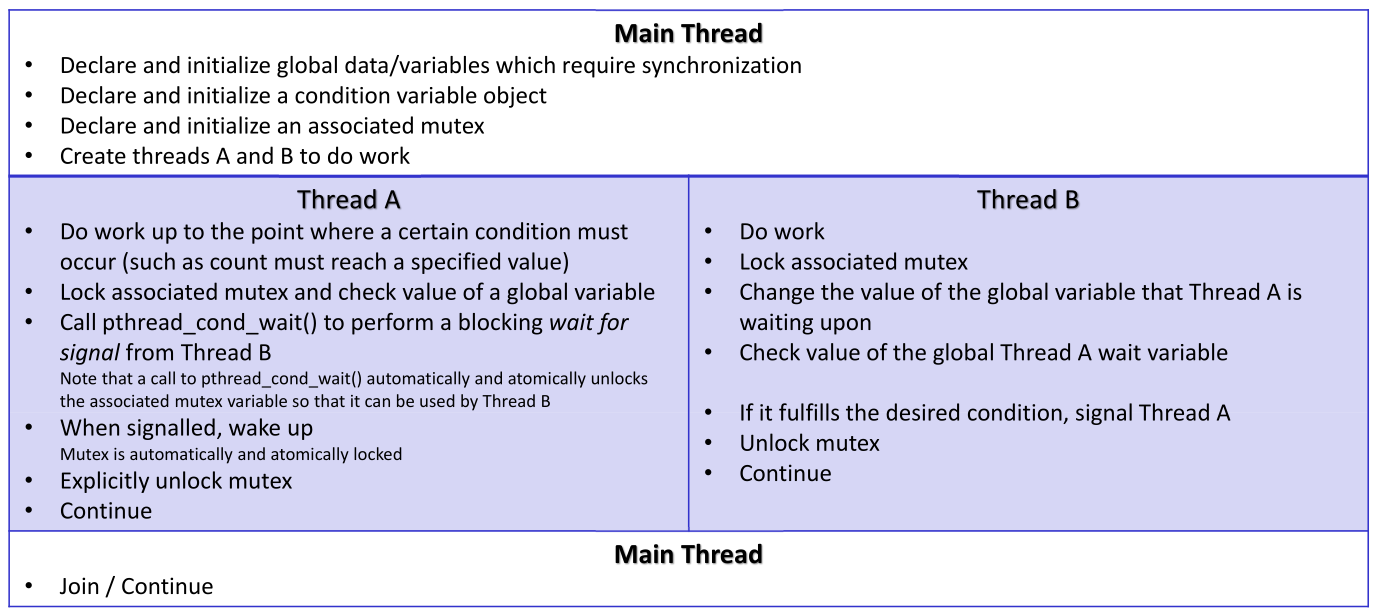
\includegraphics[width=1\textwidth]{images/Concurrency/conditionVariablesAblauf.png}
\end{centering}

\begin{multicols}{2}
  \textbf{Erzeugen}
  \\
  \begin{lstlisting}
    int pthread_cond_init(pthread_cond_t* condVar,
    const pthread_condattr_t* attr);
  \end{lstlisting}
  \begin{itemize}
    \item condVar: pointer zu condition variable
    \item attr: pointer zu \textit{pthread\_condattr\_t} Struktur, meist 0
    \item return 0 bei Erfolg, ansonsten -1
  \end{itemize}
  \vfill\null
  \columnbreak
  \textbf{Zerstören}
  \\
  \begin{lstlisting}
    int pthread_cond_destroy(pthread_cond_t* condVar);
  \end{lstlisting}
  \begin{itemize}
    \item condVar: pointer zu condition variable
    \item return 0 bei Erfolg, ansonsten -1
  \end{itemize}
\end{multicols}

\begin{multicols}{2}
  \textbf{Warten}
  \begin{lstlisting}
    int pthread_cond_wait(pthread_cond_t* condVar, pthread_mutex_t* mutex);
  \end{lstlisting}
  Diese Routine wird während dem Mutex lock aufgerufen. Der Programmierer ist für das unlock verantwortlich. 
  \vfill\null
  \columnbreak
  \textbf{Signalisieren}
  \begin{lstlisting}
    int pthread_cond_signal(pthread_cond_t* condVar);
  \end{lstlisting}
  Dieser Befehl weckt ein Thread in der Warteschlange auf.
\end{multicols}

\subsubsection{Beispiel condition variable main}
\begin{lstlisting}
enum {maxCount = 10, numThreads = 3, countLimit = 12};
volatile static int count = 0; // shared resource
static pthread_mutex_t countMutex; // the mutex
static pthread_cond_t countThresholdCv; // the condition variable
void* incCount(void* t); // count thread function
void* watchCount(void* t); // watch thread function
int main(void)
{
  int t[numThreads] = {1, 2, 3};
  pthread_t threads[numThreads];
  pthread_mutex_init(&countMutex, 0); // init mutex
  pthread_cond_init (&countThresholdCv, 0); // init condition variable
  pthread_create(&threads[0], 0, watchCount, (void*)&t[0]);
  pthread_create(&threads[1], 0, incCount, (void*)&t[1]);
  pthread_create(&threads[2], 0, incCount, (void*)&t[2]);
  for (int i = 0; i < numThreads; ++i)
    pthread_join(threads[i], 0);
  pthread_mutex_destroy(&countMutex);
  pthread_cond_destroy(&countThresholdCv);
  pthread_exit(0);
}
\end{lstlisting}

\subsubsection{Beispiel condition variable incCount}
\begin{lstlisting}
void* incCount(void* t)
{
  int myId = *(int*)t;
  printf("Starting incCount(): thread %ld\n", myId);
  for (int i = 0; i < maxCount; ++i)
  {
    pthread_mutex_lock(&countMutex); // start of critical section
    ++count;
    // Check the value of count and signal waiting thread when condition is
    // reached. Note that this occurs while mutex is locked.
    if (count == countLimit)
    pthread_cond_signal(&countThresholdCv); // signal waiting thread
    pthread_mutex_unlock(&countMutex); // end of critical section
    sleep(1); // Do some work so threads can alternate on mutex lock
  }
  pthread_exit(0);
}
\end{lstlisting}

\subsubsection{Beispiel condition variable watchCount}
\begin{lstlisting}
void* watchCount(void* t)
{
  int myId = *(int*)t;
  printf("Starting watchCount(): thread %ld\n", myId);
  // Note that pthread_cond_wait() will automatically and atomically unlock
  // mutex while it waits. Also, note that if countLimit is reached before this
  // routine is run by the waiting thread, the loop will be skipped to prevent
  // pthread_cond_wait() from never returning.
  pthread_mutex_lock(&countMutex); // start of critical section
  while (count < countLimit)
  {
    pthread_cond_wait(&countThresholdCv, &countMutex); // wait on condition
    printf("watchCount(): condition signal received.\n");
    count += 125; // updating the value of count
  }
  pthread_mutex_unlock(&countMutex); // end of critical section
  pthread_exit(0);
}
\end{lstlisting}

\subsubsection{Bounded Buffer}
\begin{tabular}{| p{8cm} |  p{8cm} |}
  \hline \textbf{Problem} & \textbf{Lösung}
  \\ Das \textit{producer-consumer} Problem (Bounded-buffer problem) ist ein Multi-Prozess synchronisationsproblem. 
  Das Problem beschreibt einen \textit{producer} und einen \textit{consumer}, welche einen gemeinsamen Buffer (Queue) nutzen. 
  Der Producer generiert Daten und legt sie um Queue ab. Der Consumer nimmt von der Queue Daten. Dabei darf der Producer keine Daten 
  mehr hinzufügen bei einer vollen Queue und der Consumer keine mehr nehmen bei einer leeren Queue.
  &
  Die Lösung für den Producer wäre die Daten zu löschen oder in sleep-Mode überzugehen. Der Consumer kann ebenfalls in den sleep-mode 
  wechseln bei einer leeren Queue.
  \\\hline
\end{tabular}

\subsection{POSIX Interprocess Communication (IPC)}
POSIX bietet folgende IPC Mechanismen für die POSIX:XSI extension an:
\begin{itemize}
  \item Message Queues in sys/msg.h
  \item Semaphores in sys/sem.h
  \item Shared Memory in sys/shm.h
\end{itemize}
Diese Mechanismen erlauben effizienten Informationsaustausch zwischen Prozessen.

\subsection{Resource Acqusition is initialisation (RAII)}
\begin{multicols}{2}
  \subsubsection{Motivation}
  \begin{itemize}
    \item Ressourcen müssen vor Gebrauch angefordert werden
    \item Nach Gebrauch der Ressourcen müssen diese wieder freigegeben werden
    \item RAII löst diese Probleme und sorgt für sauberes Anfordern und Freigeben
  \end{itemize}
  \vfill\null
  \columnbreak
  \subsubsection{Idee}
  \begin{itemize}
    \item Die Anforderung und Freigabe einer Ressource wird mit Hilfe einer Klasse implementiert
    \begin{itemize}
      \item  Konstruktor fordert die Ressource an
      \item  Destruktor gibt sie wieder frei
    \end{itemize}
    \item Ressourcen sind beispielsweise:
    \begin{itemize}
      \item Datei
      \item reservierte Speicher
      \item Semaphoren, Mutexes
      \item etc.
    \end{itemize}
    \item Die verwendete Ressource kann wie ein Objekt behandelt werden. Sobald das Objekt seine Gültigkeit 
    verliert (z. B. out-of-scope), wird durch den Destruktor die Ressource "automatisch" freigegeben.
  \end{itemize}
\end{multicols}
\newpage
\subsubsection{RAII bei Heapobjekten}
Kapsle die dynamisch erzeugte Ressource mit einem Handle-Objekt auf dem Stack.
\begin{lstlisting}
  std::shared_ptr<T> aus Header <memory>
\end{lstlisting}
Der Destruktor dieses Handle-Objekts räumt beim Verlassen des Scope automatisch auf. Das gilt auch für 
externe Ressourcen wie Files
\begin{lstlisting}
#include <memory>
void f()
{
  std::shared_ptr<Person> p(new Person("irgendwer"));
  // mach etwas mit p
  // Beim Verlassen des Blocks raeumt der Destruktor von shared_ptr
  // automatisch auf und loescht die Person
}
\end{lstlisting}

\subsubsection{RAII bei Mutex}
Sicherstellen das eine Mutex mit lock(m) angefordert wird auf jedenfall wieder freigegeben wird. 
Fehleranfälligkeit bei Exception und bei vorzeitiger Freigabe.
\begin{lstlisting}
class ResourceLock
{
  public:
  ResourceLock(pthread_mutex_t& mx) : mutex(mx) { pthread_mutex_lock(&mutex); }
  ~ResourceLock() { pthread_mutex_unlock(&mutex); }
  private:
  pthread_mutex_t& mutex; // ref to mutex of shared resource
};
void f()
{
  ...
  {
    ResourceLock lock(myMutex);
    // mach etwas in kritischem Abschnitt
    // was ist, wenn hier eine Exception geworfen wird?
  }\\!!! Hier wird lock automatisch freigegeben !!!
}
\end{lstlisting}

\newpage

\subsection{Threads in CSharp \buch{p.7}}
Prozesse und Threads aus OS-Sicht:\\
\begin{center}
{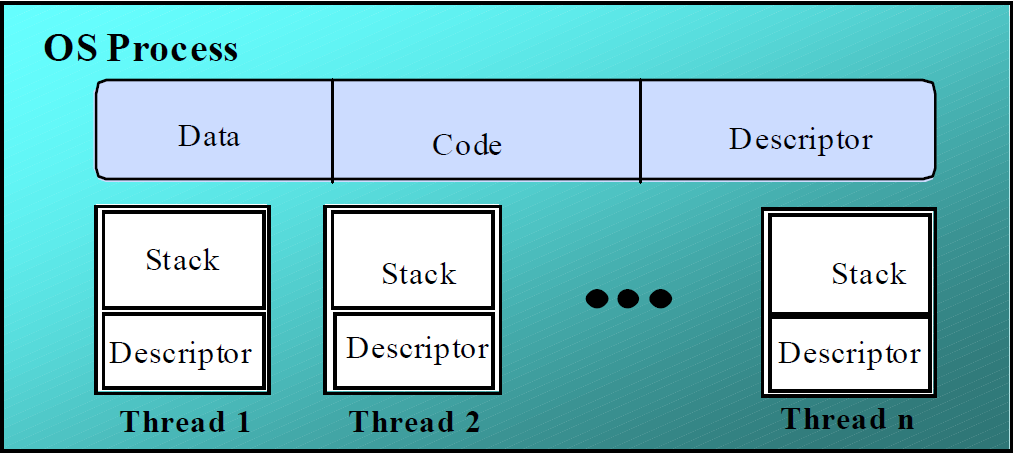
\includegraphics[width=0.5\textwidth]{images/Concurrency/ProzesseUndThreads.png}}
\end{center}
\begin{itemize}
  \item Prozess (heavyweight process):
  \begin{itemize}
    \item Code
    \item Daten
    \item Deskriptor zur Verwaltung des Prozesses durch OS (PCB, Process
    Control Block)
  \end{itemize}
  \item Thread (lightweight process):
  \begin{itemize}
    \item Teil eines Prozesses
    \item Gemeinsamer Adressraum
    \item Gemeinsame Nutzung anderer System-Ressourcen
    \item Pro Thread: Code, Stack, Deskriptor
  \end{itemize}
\end{itemize}
Ein Thread unterscheidet sich zu einem Prozess folgendermassen:\\
Man beachte: Ein Thread ist Teil eines Prozesses, das bedeutet, alles was ein
Thread inne hat, hat ein Prozess auch inne (aber NICHT umgekehrt)!\\
\begin{centering}
  \begin{tabular}{l | l}
    \hline
    \hline
    Pro Prozess vorhanden & Pro Thread vorhanden\\
    \hline
    \hline
    Adressraum & Programmzähler\\
    \hline
    Globale Variabeln & Register\\
    \hline
    Geöffnete Dateien & Stapel(Stack)\\ 
    \hline
    Kindprozesse & Zustand\\
    \hline 
    Pendente Alarme & \\
    \hline 
    Signale und Signalbehandlungsroutinen &\\
    \hline
    Buchhaltungsinformationen
  \end{tabular}
\end{centering}\\

Quasiparallelität:\\
Prozesse/Threads können folgende Zustände und Übergänge erfahren: 
\begin{center}
{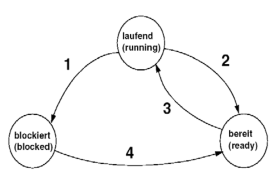
\includegraphics[width=0.5\textwidth]{images/Concurrency/Prozesszustaende.png}}
%\label{Fig: Schlechtes Beispiel für Modularisierung}
\end{center}
